\documentclass[../Thesis_AHoecherl.tex]{subfiles}

\begin{document}
    \section{Allocation of initial margin}\label{Allocation of initial margin}
    The goal of this section is to investigate if a numerical Euler allocation of \gls{ISDA SIMM} is possible.
    
    As pointed out in section \ref{sec:Euler allocation} a risk measure needs to exhibit positive homogeneity of degree 1 to be able to perform an Euler allocation.
    In a first step we can investigate by calculating ISDA SIMM for a single trade whether ISDA SIMM does exhibit positive homogeneity for a minimal example.

    For this we set up an USD Libor IRS with ten years time to maturity and a notional of 200 billion USD. This is our initial portfolio $\mathbf{u}$. ISDA SIMM would fulfill the required positive homogeneity condition if $a \rho(\mathbf{u}) = \rho(a \mathbf{u}$ for $a>0$. In figure \ref{fig:homogeneity of ISDA SIMM} $\rho(a\mathbf{u})$ is plotted for $0<a\leq 2$ in blue. 
    \begin{figure}
        \centering
        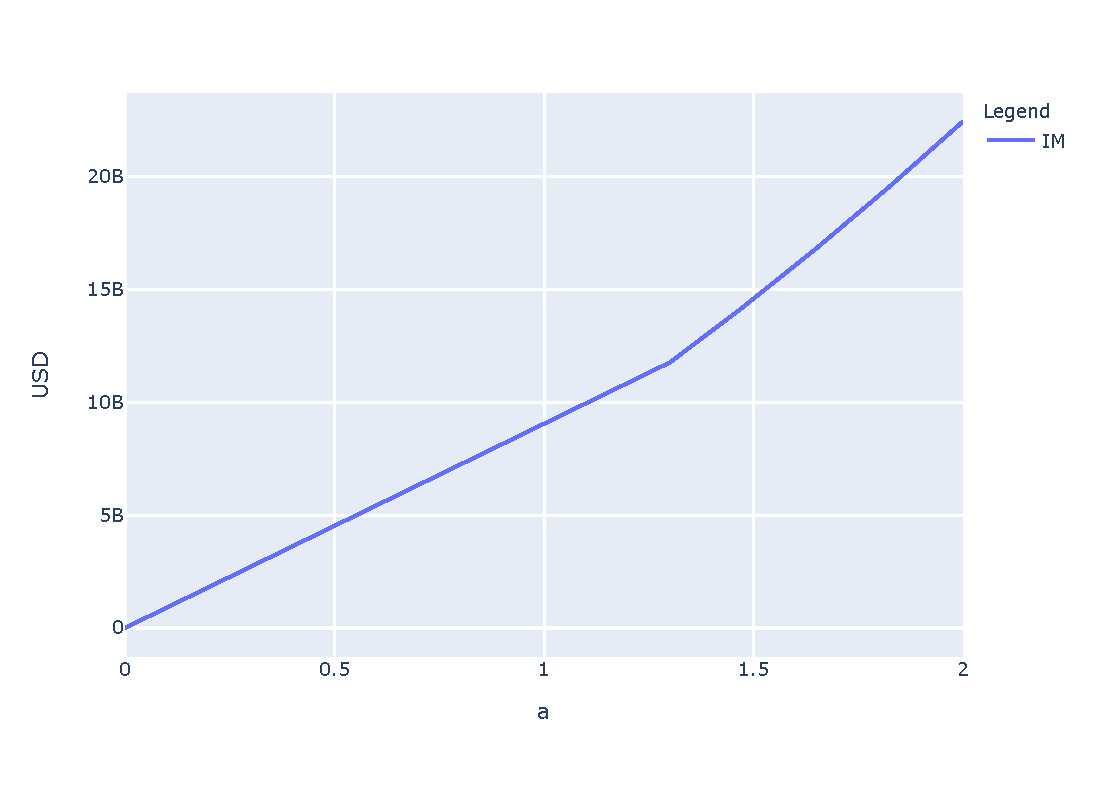
\includegraphics{Graphics/ISDA_SIMM_homogenity.pdf}
        \caption{}
        \label{fig:homogeneity of ISDA SIMM}
    \end{figure}
    The function exhibits homogeneity for $0<a<1.4$ \todo{find the exact point where homogeneity breaks} but not for higher $a$. 
    The reason for this is, that at this point the concentration risk charge of ISDA SIMM does kick in.
    The concentration risk for interest rate risks for our minimal example is defined as \cite[Article 7.b]{SIMM}
    \begin{align*}
        CR = \max\left(1,\left(\frac{\lvert\sum{s}\rvert}{T}\right)^{1/2}\right)
    \end{align*}
    with $s$ being the sensitivities against USD interest rate risk and T being 230Mn USD as specified in \cite[Article 74]{SIMM}. Due to subsequent variance-covariance aggregation the concentration risk impacts the calculated IM as
    \begin{align*}
        IM_{\text{with conc. risk}} = CR^2 \cdot IM_{\text{without conc. risk}}
    \end{align*}
    This causes the change in slope and implied loss of homogeneity visible in figure \ref{fig:homogeneity of ISDA SIMM}. If the portfolio would consist of a more diverse set of risk factors than the minimal example displayed in figure \ref{fig:homogeneity of ISDA SIMM} the associated concentration risk would kick in at different levels of $a$.
    The slope of the function would increase with each additional concentration risk not being floored at one any more. 
    
    It is important to note that as soon as the sensitivity against a single risk factor in the portfolio is above the concentration threshold the ISDA SIMM risk measure does not exhibit homogeneity anymore.

    Even a trivial example with just one trade is sufficient to show that Euler allocation does not work in the inhomogeneous part of the ISDA SIMM equation.
    For this, we compare two sample portfolios one consisting of one USD IRS with 200 bn notional and one consisting of one USD IRS with 400 bn notional.
    Critically, the second portfolio is penalized by the model since its USD IRS risk is too large. We calculate the Euler calculation with a forward finite difference approach as displayed in equation \ref{eq:forward difference}.

    Assuming that we calculate the finite difference with an $\epsilon = 0.0001$ this means that we calculate the ISDA SIMM of an IRS with 200Bn notional ($SIMM_{200Bn}$) and the ISDA SIMM of an equivalent IRS with 200.02 Bn notional ($SIMM_{200.02Bn}$) and this yields an Euler allocation to this trade as
    \begin{align*}
        \frac{SIMM_{200.02Bn} - SIMM_{200Bn}}{0.0001} = 9.04Bn
    \end{align*}
    We can see in figure \ref{fig:homogeneity of ISDA SIMM} that this value is both, the slope and the IM value at $a = 1$. The portfolios IM was correctly fully allocated to the single trade of which it consists. 
    
    However, performing the same calculation for an equivalent IRS with 400Bn notional yields
    \begin{align*}
        \frac{SIMM_{400.04Bn} - SIMM_{400Bn}}{0.0001} = 33.67Bn
    \end{align*}
    again, we can refer to figure \ref{fig:homogeneity of ISDA SIMM} to check if this is a reasonable allocation result. As $a=1$ represents the IM charge for investing 200Bn of notional in the IRS, $a=2$ represents an investment of 400Bn notional. The associated IM is just 22.44Bn - allocating 33.67Bn of the risk measure to the only trade in the portfolio is therefore clearly wrong. The Euler allocation of 33.67Bn can also be read off figure \ref{fig:homogeneity of ISDA SIMM} - it is the slope at $a=2$ times two.



    \section{Allocation of SA-CCR}\label{Allocation of SA-CCR}

    \subsection{Homogeneity of SA-CCR}

    \subsubsection{Homogeneity of C}

    To allocate \gls{SA-CCR} under consideration of margining, the available collateral $C$ is of special interest. As pointed out in table \ref{tab:Margin in SA-CCR} depending on the margining approach C can be calculated as $C = \text{VM}$ or $C = \text{VM} + \text{IM}_{\text{received}}$.

    

    \begin{figure}
        \centering
        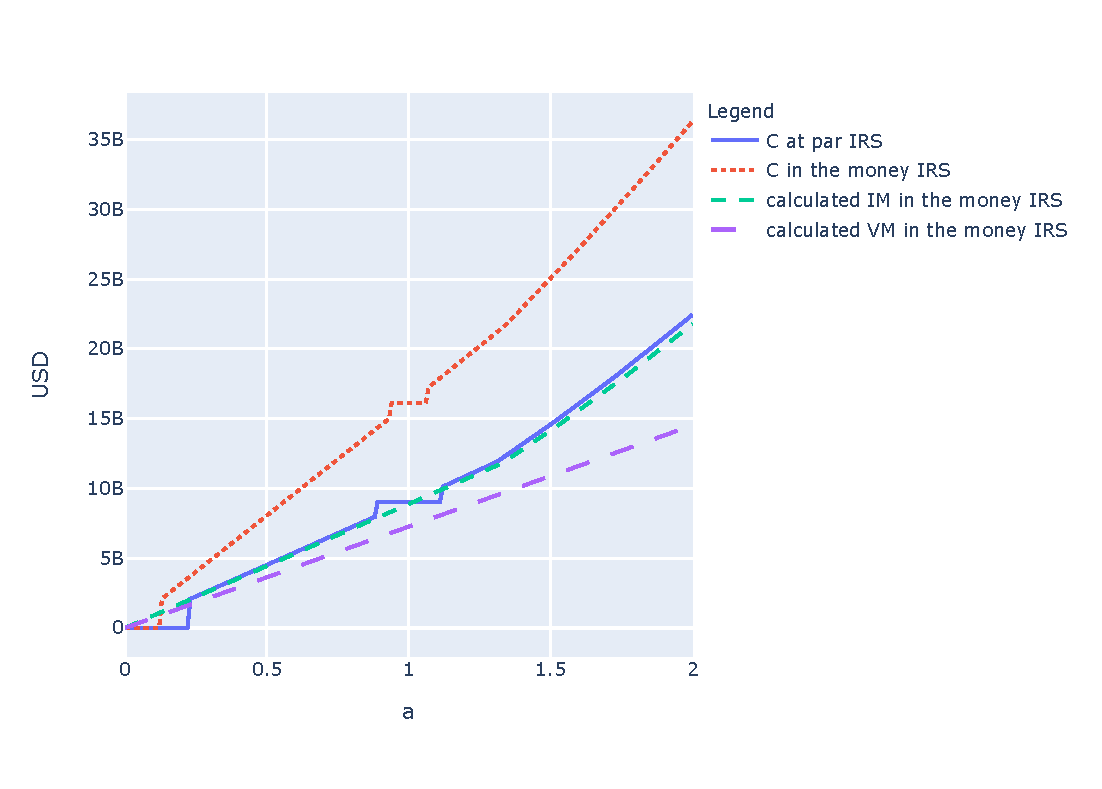
\includegraphics{Graphics/C_homogenity.pdf}
        \caption{}
        \label{fig:homogeneity of C}
    \end{figure}

    \subsection{Allocation without margining}
    \subsection{Allocation under VM collateralization}
    \subsection{Allocation under VM and IM collateralization}
\end{document}